\documentclass{article}
\usepackage{graphicx} % Required for inserting images
\graphicspath{ {./figures/} }
\usepackage[rightcaption]{sidecap}
\usepackage[table]{xcolor}
\usepackage{multirow}
\usepackage{wrapfig}
\usepackage{makecell}

\begin{document}

\section{Findings}
\label{Findings}

\subsection{JSoup Library}
\vspace{0.3cm}
\centerline{Figure 1: Test Execution Time Against Number of Containers for JSoup Library (Scaling Memory)}
\vspace{0.3cm}
\centerline{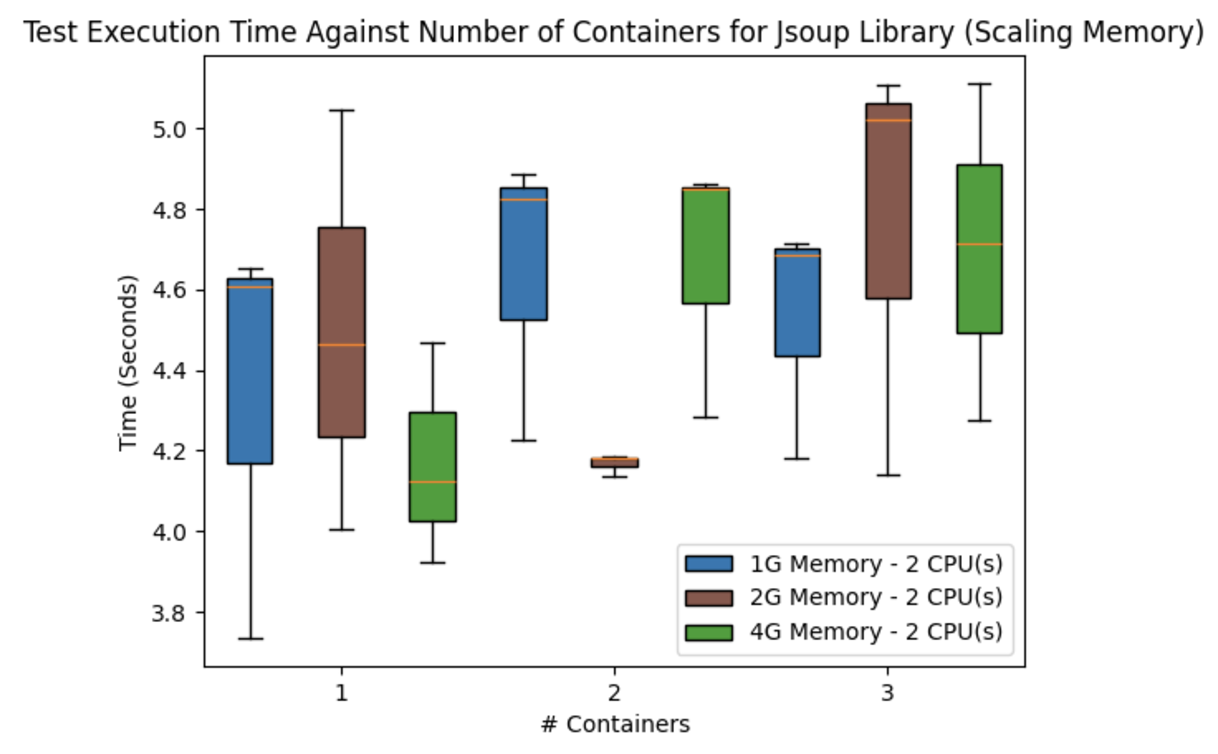
\includegraphics[width=12cm]{Figure1}}

\noindent{Figure 1 displays an insignificant improvement in test execution time as the number of containers increases. For each configuration, a one-way ANOVA test is performed to investigate if the difference in the mean execution time is statistically significant when the number of containers is increased. This indicates no evidence to suggest a difference in test execution time. The following configurations were used:}

\centerline{Table 1} 
\vspace{0.3cm}
{\centering
\begin{tabular}{|c|c|c|}
\rowcolor{gray!30}
    \hline
    Configuration & Significance (p value) & p \texttt{<} 0.05 \\
    \hline
     1G Memory – 2 CPUs & 0.6503 & No \\
     2G Memory – 2 CPUs & 0.3166 & No \\
     4G Memory – 2 CPUs & 0.1951 & No \\
     \hline
\end{tabular}
\par}

\vspace{0.4cm}
\noindent{Figure 1 also does not show a significant difference when increasing the amount of memory. Performing one-way ANOVA tests between configurations shows no statistically significant difference in the mean test execution time, regardless of the number of containers.} 

\centerline{Table 2} 
\vspace{0.3cm}
{\centering
\begin{tabular}{|c|c|c|}
\rowcolor{gray!30}
    \hline
    Container Number & Significance (p value) & p \texttt{<} 0.05 \\
    \hline
     1 & 0.6838 & No \\
     2 & 0.1284 & No \\
     3 & 0.7994 & No \\
     \hline
\end{tabular}
\par}

\newpage
\centerline{Figure 2: Test Execution Time Against Number of Containers for JSoup Library (Scaling CPUs)}
\vspace{0.3cm}
\centerline{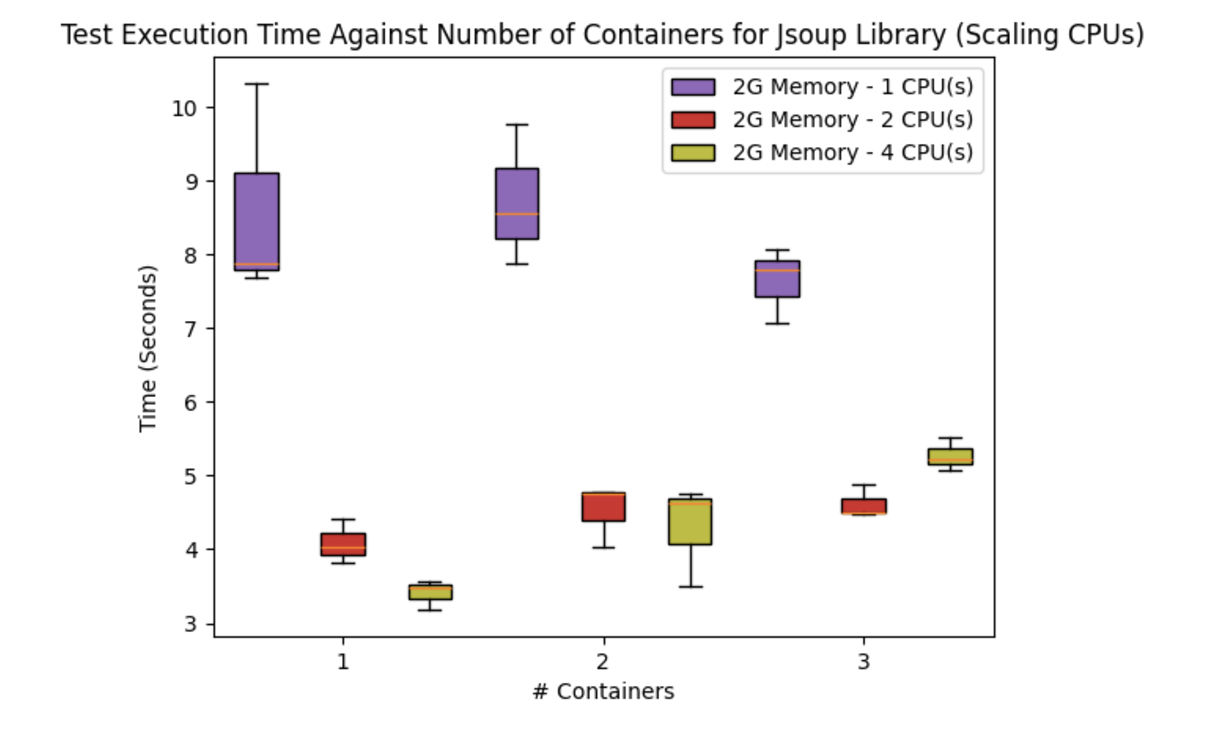
\includegraphics[width=12cm]{Figure2}}

\noindent{Figure 2 displays mixed results. When testing 2G Memory – 1 CPU, a slight improvement at 3 containers is observed, while testing 2G Memory – 2 CPUs and 2G Memory – 4 CPUs by increasing the number of containers seems to increase the test execution time. For each configuration, a one-way ANOVA test is performed to investigate if the difference in the mean execution time is statistically significant when increasing the number of containers. For scaling container CPUs, no evidence was found to suggest a difference in the test execution times, with exceptions to 2G Memory – 4 CPUs which had a p value of 0.0056.}

\centerline{Table 3} 
\vspace{0.3cm}
{\centering
\begin{tabular}{|c|c|c|}
\rowcolor{gray!30}
    \hline
    Configuration & Significance (p value) & p \texttt{<} 0.05 \\
    \hline
     2G Memory – 1 CPU & 0.4321 & No \\
     2G Memory – 2 CPUs & 0.1885 & No \\
     2G Memory – 4 CPUs & 0.0056 & Yes \\
     \hline
\end{tabular}
\par}

\vspace{0.4cm}
\noindent{Upon further investigating 2G Memory – 4 CPUs, the results suggest that increasing the number of containers increased test execution time. Performing right-tailed two-sample t-tests verified that the mean execution times increased as the number of containers increased.}

\vspace{0.2cm}
\centerline{Table 4} 
\vspace{0.3cm}
{\centering
\begin{tabular}{|c|c|c|}
\rowcolor{gray!30}
    \hline
    Container Testing & Significance (p value) & p \texttt{<} 0.05 \\
    \hline
     2 containers slower than 1 container & 0.0488 & Yes \\
     3 Containers slower than 1 Container & 0.0002 & Yes \\
     3 Containers slower than 2 Containers & 0.0402 & Yes \\
     \hline
\end{tabular}
\par}

\vspace{0.4cm}
\noindent{Figure 2 also shows some indication that increasing the number of CPUs decreased the execution time. To investigate further, one-way ANOVA tests were performed between configurations at each number of containers. This showed some statistical evidence to suggest that the mean execution times differed based on the configuration.}


\centerline{Table 5} 
\vspace{0.3cm}
{\centering
\begin{tabular}{|c|c|c|}
\rowcolor{gray!30}
    \hline
    Number of Containers & Significance (p value) & p \texttt{<} 0.05 \\
    \hline
     1 & 0.0006 & Yes \\
     2 & 0.0005 & Yes \\
     3 & 8.830e-5 & Yes \\
     \hline
\end{tabular}
\par}

\vspace{0.4cm}
\noindent{A left-tailed two-sample t-tests is performed to determine if there is a statistically significant decrease in the execution times with CPU scaling. In general, these results demonstrate that increasing the number of CPUs results in a decrease in the test execution times. However, at 2 containers and 3 containers, there is no significant decrease in test execution times when scaling from 2 to 4 CPUs with p values of 0.3268 and 0.9886, respectively. Moreover, in the case of 3 containers, a significant increase in test execution times with a p value of 0.0114 can be observed.}

\centerline{Table 6} 
\vspace{0.3cm}
{\centering
\begin{tabular}{|c|c|c|c|}
\rowcolor{gray!30}
    \hline
     Number of Containers & Comparison & Significance (p value) & p \texttt{<} 0.05 \\
     \hline
     \multirow{3}{*}{1} & \multicolumn{1}{|c|}{2 CPUs faster than 1 CPU} & \multicolumn{1}{c|}                    {0.0032} & \multicolumn{1}{c|}{Yes} \\\cline{2-4}
                        & \multicolumn{1}{|c|}{4 CPUs faster than 1 CPU} & \multicolumn{1}{c|}{0.0018} & \multicolumn{1}{c|}{Yes} \\\cline{2-4}
                        & \multicolumn{1}{|c|}{4 CPUs faster than 2 CPUs} & \multicolumn{1}{c|}{0.0151} & \multicolumn{1}{c|}{Yes} \\\Xhline{1pt} 

    \multirow{3}{*}{2} & \multicolumn{1}{|c|}{2 CPUs faster than 1 CPU} & \multicolumn{1}{c|}                      {0.0012} & \multicolumn{1}{c|}{Yes} \\\cline{2-4}
                        & \multicolumn{1}{|c|}{4 CPUs faster than 1 CPU} & \multicolumn{1}{c|}{0.0015} & \multicolumn{1}{c|}{Yes} \\\cline{2-4}
                        & \multicolumn{1}{|c|}{4 CPUs faster than 2 CPUs} & \multicolumn{1}{c|}{0.3268} & \multicolumn{1}{c|}{No} \\\Xhline{1pt} 

    \multirow{3}{*}{3} & \multicolumn{1}{|c|}{2 CPUs faster than 1 CPU} & \multicolumn{1}{c|}                      {0.0003} & \multicolumn{1}{c|}{Yes} \\\cline{2-4}
                        & \multicolumn{1}{|c|}{4 CPUs faster than 1 CPU} & \multicolumn{1}{c|}{0.0009} & \multicolumn{1}{c|}{Yes} \\\cline{2-4}
                        & \multicolumn{1}{|c|}{4 CPUs faster than 2 CPUs} & \multicolumn{1}{c|}{0.9886} & \multicolumn{1}{c|}{No} \\\hline
\end{tabular}
\par}

\newpage
\subsection{Guava Library}
\vspace{0.3cm}
\centerline{Figure 3: Test Execution Time Against Number of Containers for Guava Library (Scaling Memory)}
\vspace{0.3cm}
\centerline{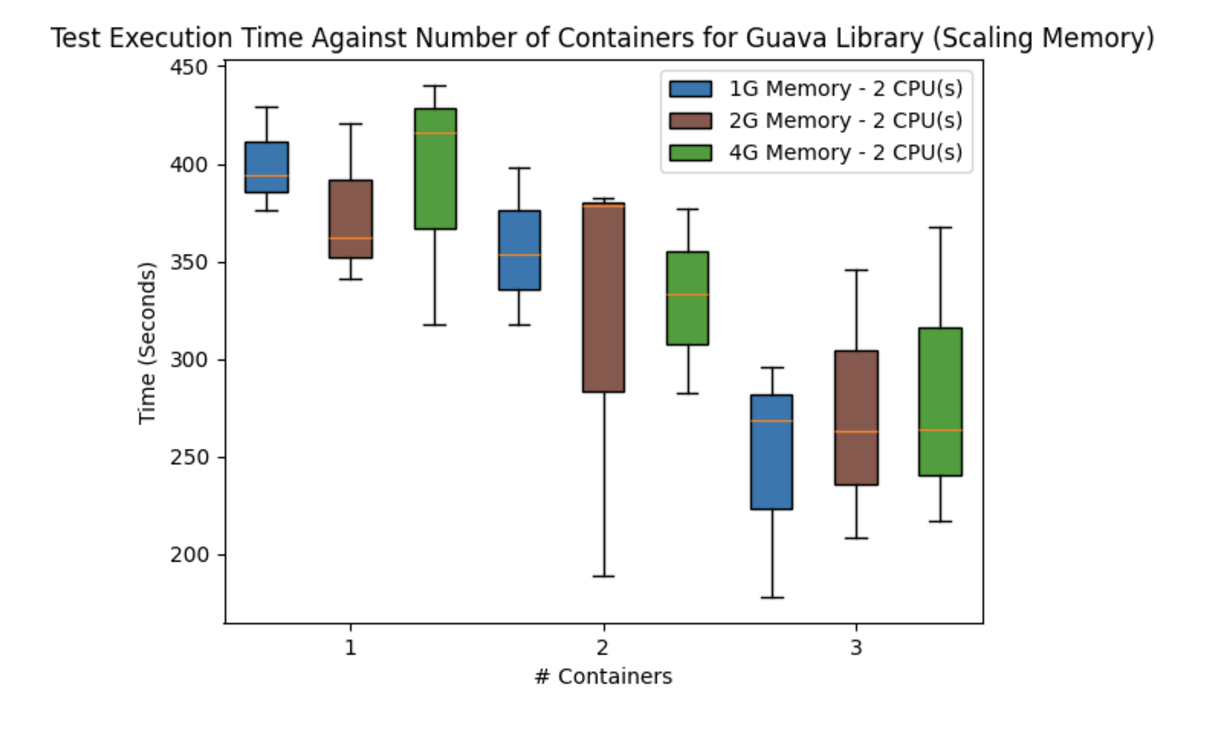
\includegraphics[width=12cm]{Figure3}}

\noindent{Figure 3 displays a downward trend as the number of containers increases. To verify this observation, one-way ANOVA tests are performed to determine the significance of the differences in test execution time as the number of containers increased.}

\centerline{Table 7} 
\vspace{0.3cm}
{\centering
\begin{tabular}{|c|c|c|}
\rowcolor{gray!30}
    \hline
    Configuration & Significance (p value) & p \texttt{<} 0.05 \\
    \hline
     1G Memory – 2 CPUs & 0.0154 & Yes \\
     2G Memory – 2 CPUs & 0.3463 & No \\
     4G Memory – 2 CPUs & 0.1977 & No \\
     \hline
\end{tabular}
\par}

\vspace{0.4cm}
\noindent{It was determined that only in the case of 1G Memory – 2 CPUs, is there a statistically significant difference when the number of containers is increased. To further investigate these differences, left-tailed two-sample t-tests are performed to determine the significance of the changes when increasing the number of containers. No significant decrease in test execution times was found when moving from 1 container to 2 containers, however, when moving from 1 container to 3 containers and 2 containers to 3 containers, there was a significant decrease with p values of 0.0085 and 0.0311 respectively.}

\newpage
\centerline{Table 8} 
\vspace{0.3cm}
{\centering
\begin{tabular}{|c|c|c|}
\rowcolor{gray!30}
    \hline
    Comparison & Significance (p value) & p \texttt{<} 0.05 \\
    \hline
     2 containers faster than 1 container & 0.0970 & No \\
     3 containers faster than 1 container & 0.0085 & Yes \\
     3 containers faster than 2 containers & 0.0311 & Yes \\
     \hline
\end{tabular}
\par}

\vspace{0.4cm}
\noindent{Figure 3, much like Figure 1, shows insignificant evidence that increasing the amount of memory reduced test execution times. One-way ANOVA tests were performed to determine if there was any statistically significant difference in test executions times. No evidence was found suggesting increasing memory improved test execution times regardless of the number of containers.}

\vspace{0.2cm}
\centerline{Table 9} 
\vspace{0.3cm}
{\centering
\begin{tabular}{|c|c|c|}
\rowcolor{gray!30}
    \hline
    Number of Containers & Significance (p value) & p \texttt{<} 0.05 \\
    \hline
     1 & 0.8061 & No \\
     2 & 0.8027 & No \\
     3 & 0.8180 & No \\
     \hline
\end{tabular}
\par}

\vspace{0.4cm}
\centerline{Figure 4: Test Execution Time Against Number of Containers for Guava Library (Scaling CPUs)}
\vspace{0.3cm}
\centerline{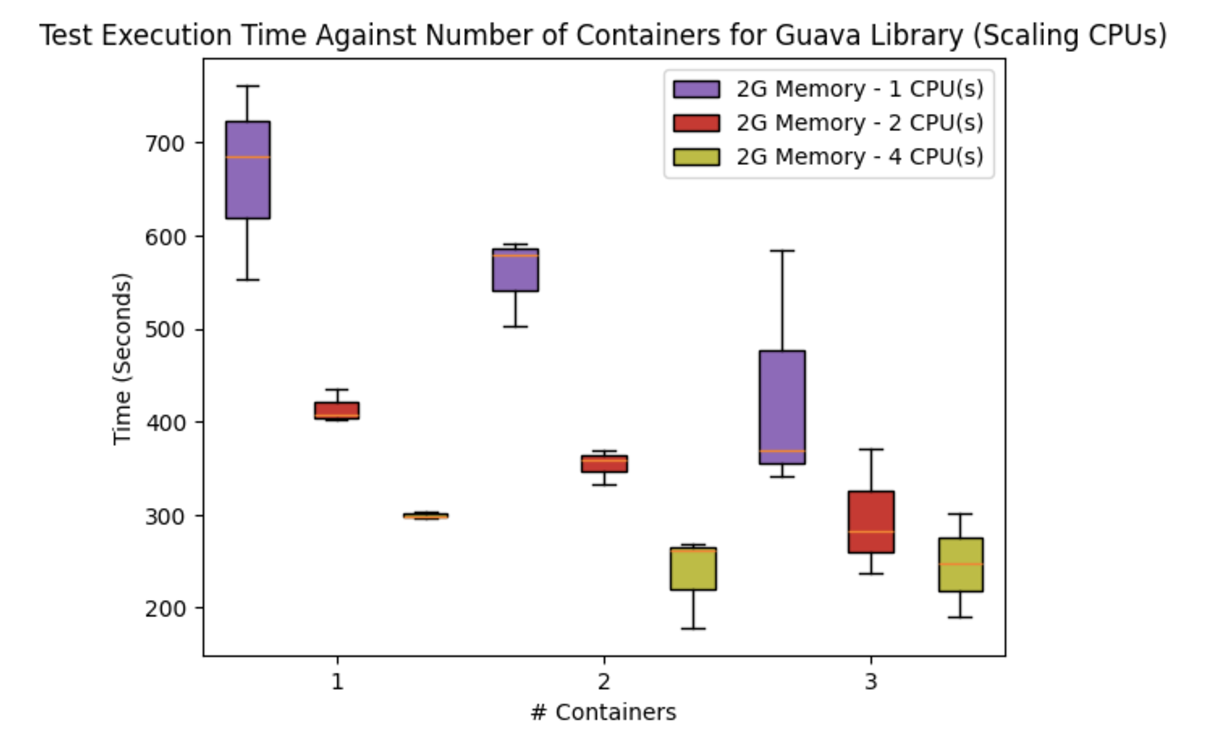
\includegraphics[width=12cm]{Figure4}}

\noindent{Figure 4 displays some significant decrease in the execution times. One-way ANOVA tests were performed to determine the significance of the differences in execution times as the number of containers increased for each configuration. Only significant differences for 2G Memory and 2 CPUs have been observed.}

\newpage
\centerline{Table 10} 
\vspace{0.3cm}
{\centering
\begin{tabular}{|c|c|c|}
\rowcolor{gray!30}
    \hline
    Configuration & Significance (p value) & p \texttt{<} 0.05 \\
    \hline
     2G Memory – 1 CPU & 0.0781 & No \\
     2G Memory – 2 CPUs & 0.0372 & Yes \\
     2G Memory – 4 CPUs & 0.2405 & No \\
     \hline
\end{tabular}
\par}

\vspace{0.4cm}
\noindent{To further investigate the differences found at 2G Memory and 2 CPUs, left-tailed two-sample t-tests were performed to determine if there was a presence of statistically significant decreases in test execution time as the number of containers increased. The results showcase that increasing from 1 container to 2 or 3 containers produces improved execution times with p values of 0.0075 and 0.0215, but not when increasing from 2 to 3 containers with a p value of 0.1158.}

\centerline{Table 11} 
\vspace{0.3cm}
{\centering
\begin{tabular}{|c|c|c|}
\rowcolor{gray!30}
    \hline
    Comparison & Significance (p value) & p \texttt{<} 0.05 \\
    \hline
     2 containers faster than 1 container & 0.0075 & Yes \\
     3 containers faster than 1 container & 0.0215 & Yes \\
     3 containers faster than 2 containers & 0.1158 & No \\
     \hline
\end{tabular}
\par}

\vspace{0.4cm}
\noindent{Additionally, Figure 4 shows that regardless of the number of containers, the test execution time can be improved by increasing the number of CPUs. One-way ANOVA tests were performed for each number of containers to determine any significant differences in test execution times. At 1 and 2 containers, the data suggests that increasing the number of CPUs had an impact on the execution time, with p values of 0.0009 and 0.0002, respectively. However, for 3 containers, no significant difference is observed.}

\vspace{0.2cm}
\centerline{Table 12} 
\vspace{0.3cm}
{\centering
\begin{tabular}{|c|c|c|}
\rowcolor{gray!30}
    \hline
    Number of Containers & Significance (p value) & p \texttt{<} 0.05 \\
    \hline
     1 & 0.0009 & Yes \\
     2 & 0.0002 & Yes \\
     3 & 0.1101 & No \\
     \hline
\end{tabular}
\par}

\vspace{0.4cm}
\noindent{To further investigate the differences found in test execution time for 1 and 2 containers, left-tailed two-sample t-tests were performed to determine the presence of significant decreases in test execution times as the number of CPUs increase. With both numbers of containers, the data suggests that increasing the number of CPUs results in lower test execution times.}

\newpage
\centerline{Table 13} 
\vspace{0.3cm}
{\centering
\begin{tabular}{|c|c|c|c|}
\rowcolor{gray!30}
    \hline
     Number of Containers & Comparison & Significance (p value) & p \texttt{<} 0.05 \\
     \hline
     \multirow{3}{*}{1} & \multicolumn{1}{|c|}{2 CPUs faster than 1 CPU} & \multicolumn{1}{c|}                    {0.0076} & \multicolumn{1}{c|}{Yes} \\\cline{2-4}
                        & \multicolumn{1}{|c|}{3 CPUs faster than 1 CPU} & \multicolumn{1}{c|}{0.0019} & \multicolumn{1}{c|}{Yes} \\\cline{2-4}
                        & \multicolumn{1}{|c|}{3 CPUs faster than 2 CPUs} & \multicolumn{1}{c|}{0.0002} & \multicolumn{1}{c|}{Yes} \\\Xhline{1pt} 

    \multirow{3}{*}{2} & \multicolumn{1}{|c|}{2 CPUs faster than 1 CPU} & \multicolumn{1}{c|}                      {0.0012} & \multicolumn{1}{c|}{Yes} \\\cline{2-4}
                        & \multicolumn{1}{|c|}{3 CPUs faster than 1 CPU} & \multicolumn{1}{c|}{0.0006} & \multicolumn{1}{c|}{Yes} \\\cline{2-4}
                        & \multicolumn{1}{|c|}{3 CPUs faster than 2 CPUs} & \multicolumn{1}{c|}{0.0096} & \multicolumn{1}{c|}{Yes} \\\Xhline{1pt} 
\end{tabular}
\par}

\end{document}
